\documentclass[mat1, tisk]{fmfdelo}
% \documentclass[fin1, tisk]{fmfdelo}
% Če pobrišete možnost tisk, bodo povezave obarvane,
% na začetku pa ne bo praznih strani po naslovu, …

%%%%%%%%%%%%%%%%%%%%%%%%%%%%%%%%%%%%%%%%%%%%%%%%%%%%%%%%%%%%%%%%%%%%%%%%%%%%%%%
% METAPODATKI
%%%%%%%%%%%%%%%%%%%%%%%%%%%%%%%%%%%%%%%%%%%%%%%%%%%%%%%%%%%%%%%%%%%%%%%%%%%%%%%

% - vaše ime
\avtor{Jaša Knap}

% - naslov dela v slovenščini
\naslov{Kratki zakoni v grupah}

% - naslov dela v angleščini
\title{Short group laws}

% - ime mentorja/mentorice s polnim nazivom:
%   - doc.~dr.~Ime Priimek
%   - izr.~prof.~dr.~Ime Priimek
%   - prof.~dr.~Ime Priimek
%   za druge variante uporabite ustrezne ukaze
\mentor{doc.~dr.~Urban Jezernik}
% \somentor{...}
% \mentorica{...}
% \somentorica{...}
% \mentorja{...}{...}
% \somentorja{...}{...}
% \mentorici{...}{...}
% \somentorici{...}{...}

% - leto diplome
\letnica{2024} 

% - povzetek v slovenščini
%   V povzetku na kratko opišite vsebinske rezultate dela. Sem ne sodi razlaga
%   organizacije dela, torej v katerem razdelku je kaj, pač pa le opis vsebine.

% Dvočrkovni zakon v grupi $G$ je abstrakten produkt elementov $x$, $y$ ter njunih inverzov $x^{-1}$ in $y^{-1}$, ki ima lastnost, da za vsako zamenjavo $x$ in $y$ s konkretnima
% elementoma $g, h \in G$ dobimo rezultat $1 \in G$. Na primer beseda $xyx^{-1}y^{-1}$ je zakon v grupi natanko tedaj, ko je grupa Abelova. Tema diplomske naloge je ocenjevanje asimtotske rasti dolžine najkrajših netrivialnih zakonov za specifične družine grup, še posebej družine $\operatorname{PSL}_2(q)$ in družine nilpotentnih grup določenega razreda nilpotentnosti. Proti koncu se naloga dotakne tudi računalniškega iskanja zakonov. 

\povzetek{TODO}

% - povzetek v angleščini
\abstract{TODO}

% - klasifikacijske oznake, ločene z vejicami
%   Oznake, ki opisujejo področje dela, so dostopne na strani https://www.ams.org/msc/
\klasifikacija{20, 05C81} % TODO

% - ključne besede, ki nastopajo v delu, ločene s \sep
\kljucnebesede{...\sep ...} % TODO

% - angleški prevod ključnih besed
\keywords{...\sep ...} % angleški prevod ključnih besed TODO

% - angleško-slovenski slovar strokovnih izrazov
% TODO
\slovar{
% \geslo{angleški izraz}{slovenski izraz}
% ...
}

% - ime datoteke z viri (vključno s končnico .bib), če uporabljate BibTeX
\literatura{literatura.bib}

%%%%%%%%%%%%%%%%%%%%%%%%%%%%%%%%%%%%%%%%%%%%%%%%%%%%%%%%%%%%%%%%%%%%%%%%%%%%%%%
% DODATNE DEFINICIJE
%%%%%%%%%%%%%%%%%%%%%%%%%%%%%%%%%%%%%%%%%%%%%%%%%%%%%%%%%%%%%%%%%%%%%%%%%%%%%%%

% naložite dodatne pakete, ki jih potrebujete
% \usepackage{...}

\usepackage{tikz}

% deklarirajte vse matematične operatorje, da jih bo LaTeX pravilno stavil
% \DeclareMathOperator{\...}{...}

% vstavite svoje definicije ...
% \newcommand{\...}{...}

%%%%%%%%%%%%%%%%%%%%%%%%%%%%%%%%%%%%%%%%%%%%%%%%%%%%%%%%%%%%%%%%%%%%%%%%%%%%%%%
% ZAČETEK VSEBINE
%%%%%%%%%%%%%%%%%%%%%%%%%%%%%%%%%%%%%%%%%%%%%%%%%%%%%%%%%%%%%%%%%%%%%%%%%%%%%%%

\begin{document}

\section{Uvod}

% TODO tale uvod je treba še kar lepo urediti, da bo v smiselni obliki
% treba je obrazložiti kaj je sploh poanta diplome

Dvočrkovni zakon v grupi $G$ je abstrakten produkt elementov $x$, $y$ ter njunih inverzov $x^{-1}$ in $y^{-1}$, ki ima lastnost, da za vsako zamenjavo $x$ in $y$ s konkretnima
elementoma $g, h \in G$ dobimo rezultat $1 \in G$.

\begin{opomba}
Definicijo $n$-črkovnih zakonov dobimo tako, da v zgornji definiciji elementa $x$, $y$ (in njuna inverza) nadomestimo z elementi $x_1, x_2, \ldots, x_n$ (in njihovimi inverzi),
ki jih zamenjujemo s konkretnimi elementi $g_1, g_2, \ldots, g_{n} \in G$.
\end{opomba}

\noindent
Zakonu $1$ pravimo trivialni zakon, ki v kontekstu raziskovanja zakonov ni posebej zanimiv. Najosnovnejši primer netrivialnega zakona se pojavi pri Abelovih grupah, kjer za poljubna elementa $x,y \in  G$ velja $xy = yx$, kar je ekvivalentno
zahtevi \begin{equation*}
xyx^{-1}y^{-1} = [x,y] = 1.
\end{equation*}

\noindent
Grupa $G$ je torej Abelova natanko tedaj, ko je štiričrkovna beseda $xyx^{-1}y^{-1}$ v njej zakon. 


\section{Osnovni pojmi}

Definicijo zakona \href{def_zakon_osnovna} lahko bolj formalno zapišemo s pomočjo prostih grup.

\begin{definicija}
\label{def_prosta_grupa}
Naj bo $S$ množica. Grupa $F(S)$ je (do izomorfizma natančno) enolična grupa z lastnostjo, da za poljubno grupo $G$ in poljubno preslikavo
$\varphi: S \to G$ obstaja natanko ena razširitev $\varphi: F(S) \to G$, ki je hkrati homomorfizem grup. 
\end{definicija}

\begin{opomba}
Za poljubni množici $S$ in $T$ velja $F(S) \cong F(T)$ natanko tedaj, ko $\lvert S \rvert = \lvert T \rvert$. Zato lahko v primeru končne množice $\lvert S \rvert = k$ govorimo o 
prosti grupi ranga $k$, ki jo označimo z $F_k$.
\end{opomba}

\noindent
V viru (TODO, morda \cite[str.~4]{Lyndon_Schupp_2015}) je natančno razloženo znano dejstvo, da lahko elemente proste grupe $F(S)$ predstavimo v obliki okrajšanih besed,
torej besed oblike $w = s_1 \cdots s_n$, kjer je $s_i \in S \cup S^{-1}$ za $i = 1, \ldots, n$ in $s_i \neq s_{i+1}^{-1}$ za $i = 1, \ldots, n-1$. Tu je $S^{-1} = \left\{ s^{-1}  \middle|\, s \in  S \right\}$.
Z upoštevanjem tega dejstva lahko elementom proste grupe $F(S)$ določimo dolžino.

\begin{definicija}
\label{def_dolzina_besede}
Naj bo $w \in  F(S)$ element proste grupe nad množico $S$ in naj bo njegova okrajšana oblika $w = s_1 \cdots s_n$. Potem številu $n$ pravimo dolžina (besede) $w$ in pišemo $l(w) = n$.
\end{definicija}

\noindent
Zdaj definiramo izginjajočo množico besede $w$ v grupi $G$.

\begin{definicija}
\label{def_izginjajoca_mnozica}
Naj bo $w \in  F_k$. Potem množico \begin{equation*}
Z(G, w) := \left\{ (g_1, .., g_{k}) \in  G^{k}  \middle|\, w(g_1, \ldots, g_{k}) = 1 \right\} 
\end{equation*}  
imenujemo izginajoča množica besede $w$ v grupi $G$. Tu $1$ označuje enoto v grupi $G$, $w(g_1, \ldots, g_{k})$ pa sliko elementa $w \in F_k = \langle a_{1}, \ldots , a_k \rangle$ s homomorfizmom,
induciranim s preslikavo $\varphi: a_{i} \mapsto g_{i}$ za $i = 1,\ldots, n$ v skladu z definicijo \href{def_prosta_grupa}.  
\end{definicija}

\indent
Zdaj lahko natančno formuliramo definicjo zakona.

\begin{definicija}
\label{def_zakon_formalna}
Beseda $w \in F_k$ je $k$-črkovni zakon v grupi $G$, če je $Z(G, w) = G^{k}$. Alternativno, beseda $w \in F_k$ je $k$-črkovni zakon v grupi $G$, če jo vsak homomorfizem $\varphi: F_k \to G$ slika v enoto $1 \in G$.   
\end{definicija}

Ta definicija nam omogoča vpogled v strukturo zakonov. Naj $K(k) \subseteq F_k$ označuje množico $k$-črkovnih zakonov. Potem v luči prejšnje definicije velja
\begin{equation*}
K(k)  = \bigcap_{\varphi: F_k \to G} \operatorname{ker}(\varphi).   
\end{equation*}  
Ta množica je končni presek edink v $G$ in posledično tudi sama edinka. Še več, invariantna je za vsak avtomorfizem $\alpha: F_k \to  F_k$, saj
\begin{equation*}
    K(k)  = \bigcap_{\varphi: F_k \to G} \operatorname{ker}(\varphi) = \bigcap_{\varphi: F_k \to G} \operatorname{ker}(\varphi \circ \alpha). 
\end{equation*}  
To je preprosta posledica dejstva, da $\varphi$ preteče grupo $\operatorname{Hom}(F_k, G)$ natanko tedaj, ko jo preteče $\varphi \circ \alpha$.     

\begin{lema}
\label{lem_koncni_indeks_koncnega_preseka}
Naj bo $G$ grupa ter $H_1, \ldots, H_n$ njene podgrupe končnega indeksa, torej $[G: H_i] < \infty$ za $i = 1, \ldots, n$. Potem je tudi $\bigcap_{i = 1}^{n} H_i$ podgrupa končnega indeksa v $G$ in velja
\begin{equation*}
\left[ G: \bigcap_{i = 1}^{n} H_i \right]  \le \prod_{i=1}^{n} [G: H_i].  
\end{equation*} 
\end{lema}

\begin{dokaz}
TODO
\end{dokaz}
Z uporabo te leme direktno sledi, da je grupa $K(k)$ podgrupa končnega indeksa v $F_k$. To dejstvo bo še posebej pobmembno pri iskanju zakonov z računalnikom.

\begin{definicija}
\label{def_ozina}
Število \begin{equation*}
\text{girth}_{k}(G) := \min \left\{ l(w)  \middle|\,  w \in F_k \setminus \left\{ 1\right\} \text{ je zakon v } G  \right\} \cup \left\{ \infty\right\} 
\end{equation*}  
je $k$-črkovna dolžina grupe $G$.  
\end{definicija}

Ime ožina je smiselno v kontekstu definicije Cayleyjevega grafa grupe.

\begin{definicija}
\label{def_cayleyev_graf}
Naj bo $G$ grupa in $S \subseteq G$ njena podmnožica, za katero velja $S = S^{-1}$. Potem $\operatorname{Cay}(G, S)$ označuje graf z množico vozlišč $V = G$ in povezavami
$E = \left\{ (p, q) \middle|\, p^{-1}q \in  S \right\}$. Imenujemo ga Cayleyjev graf grupe $G$, generiran z množico $S$.  
\end{definicija}

\begin{opomba}
Pogoj $S = S^{-1}$ nam pove, da je $\operatorname{Cay}(G, S)$ res pravi graf in ne zgolj usmerjen. Imamo namreč \begin{equation*}
(p,q) \in  E \iff p^{-1}q \iff q^{-1}p \iff (q,p) \in  E.
\end{equation*}  
\end{opomba}

\begin{primer}
Na spodnjih slikah imamo Cayleyjev graf grupe $D_{10}$ (diedrske grupe z $10$ elementi) za različni generatorski množici.
TODO nariši grafa, enega imaš iz predstaviltve, drugega postavi zraven
\begin{center}
    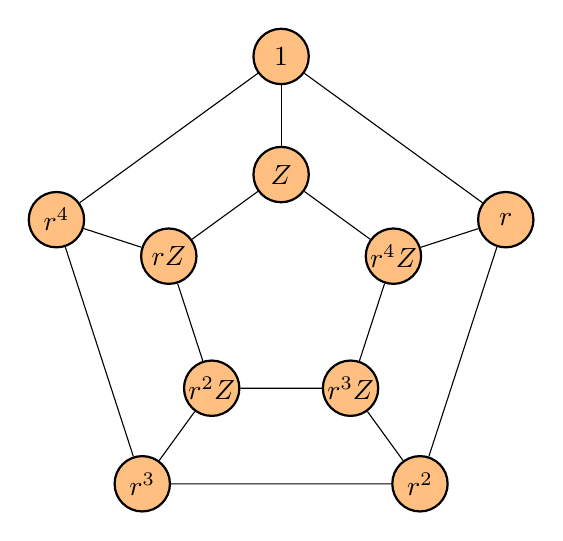
\begin{tikzpicture}[rotate=90, scale=1.5]
    \tikzset{vertex/.style={draw, thick, circle, fill=orange!50, minimum size=20pt, inner sep=0pt}}
    
    \node[vertex] (v1) at (-0*360/5:1) {$Z$};
    \node[vertex] (v2) at (-0*360/5:2) {$1$};
    \node[vertex] (v3) at (-1*360/5:1) {$r^4Z$};
    \node[vertex] (v4) at (-1*360/5:2) {$r$};
    \node[vertex] (v5) at (-2*360/5:1) {$r^3Z$};
    \node[vertex] (v6) at (-2*360/5:2) {$r^2$};
    \node[vertex] (v7) at (-3*360/5:1) {$r^2Z$};
    \node[vertex] (v8) at (-3*360/5:2) {$r^3$};
    \node[vertex] (v9) at (-4*360/5:1) {$rZ$};
    \node[vertex] (v10) at (-4*360/5:2) {$r^4$};
    
    \draw (v1) -- (v2);
    \draw (v1) -- (v3);
    \draw (v2) -- (v4);
    \draw (v3) -- (v4);
    \draw (v3) -- (v5);
    \draw (v4) -- (v6);
    \draw (v5) -- (v6);
    \draw (v5) -- (v7);
    \draw (v6) -- (v8);
    \draw (v7) -- (v8);
    \draw (v1) -- (v9);
    \draw (v7) -- (v9);
    \draw (v2) -- (v10);
    \draw (v8) -- (v10);
    \draw (v9) -- (v10);
    \end{tikzpicture}
    \end{center}
\end{frame}

\end{primer}


Izkaže se, da so najbolj zanimivi zakoni za obravnavo dvočrkovni. To utemeljimo z dokazom naslednje trditve.

\begin{trditev}
\label{trd_vlozitev_proste_grupe}
 Obstaja vložitev $F_{2 \cdot 3^{k}} = \langle x_1, \ldots, x_{2 \cdot 3^{k}} \rangle$ v $F_2 = \langle x,y \rangle $, da velja $l(x_i) = 2k + 1$, kjer $l(w)$ označuje dolžino besede $w \in F_2 = \langle x,y \rangle$. 
\end{trditev}
\begin{dokaz}
    TODO, treba je še prej definirati Schreierjev graf in fundamentalno grupo grafa
\end{dokaz}



\section{Komutatorska in razširitvena lema}

~\cite{Schneider_2016}

\section{Nilpotentne in rešljive grupe}

\cite{Schneider_2016}, \cite{Bradford_Thom_2022}, \cite{Kozma_Thom_2016}


\section{Enostavne grupe}

\cite{Schneider_2016}

\section{Grupe $\operatorname{PSL}_2(q)$ in $\operatorname{PSL}_n(q)$}

\cite{Bradford_Thom_2022}, \cite{Schneider_2016}

\section{Simetrične grupe}

\cite{Kozma_Thom_2016}

\section{Iskanje zakonov z računalnikom}

\subsection{Iskanje zakonov za grupe $\operatorname{PSL}_2(q)$} %

To je tisto kar sem že sprogramiral.

\subsection{Iskanje generatorjev zakonov za nilpotentne grupe}

\cite{Cocke_2020}, še posebej pa \cite{Chilebus_Cocke_Ho_2024}

\section{Zaključek}
% ...


% \bibliographystyle{plain}
% \selectlanguage{slovene}
% \begin{thebibliography}{5}
%     \bibitem{Kozma_Thom_2016}
%     G.~Kozma in A.~Thom, \emph{Divisibility and laws in finite simple groups}, Mathematische Annalen \textbf{364 (1-2)} (2016) 79--95. 
%      \bibitem{Schneider_2016}
%      J.~Schneider, \emph{On the length of group laws}, magistrsko delo, Department of mathematics, Technische Universität Dresden, 2016.
%      \bibitem{Bradford_Thom_2022}
%      H.~Bradford in A.~Thom, \emph{Short laws for finite groups of Lie type}, verzija 5.~10.~2022 [ogled 29.~2.~2024], dostopno na \url{https://arxiv.org/abs/1811.05401}.
%      \bibitem{Bradford_Jakob_Schneider_Thom_2023}
%      H.~Brandford, J.~Schneider in A.~Thom, \emph{Non-singular word maps for linear groups}, verzija 7.~11.~2023 [ogled 29.~2.~2024], dostopno na \url{https://arxiv.org/abs/2311.03981}. 
%      \bibitem{Amir_Blachar_Gerasimova_Kozma_2023}
%      G.~Amir, G.~Blachar, M.~Gerasimova in G.~Kozma, \emph{Probabilistic laws on infinite groups}, verzija 18.~4.~2023 [ogled 29.~2.~2024], dostopno na \url{https://arxiv.org/abs/2304.09144}. 
%     \end{thebibliography}

\end{document}
